\section{Background and Modeling}
In this section we breifly describe the general architecture of FPGAs, the design flow in partial reconfiguration (PR) and the assumptions that led to the fromulation of PR floorplanning problem as a MILP problem. This work is based on the 7 series FPGA family from Xilinx. \\

\subsection{FPGA Architecture and Partial-Reconfiguration}

The configurable fabric of Xilinx FPGAs is divided into quadrants named clock regions. Within each clock region there are columns of different configurable resources such as CLBs, BRAMs or DSPs.  Resources within a clock region share the same clock. A single column in a clock region is referred to as a tile. The number of resources in a tile varies depending on the device family. For example in Virtex 7z a CLB tile contains 50 clbs a BRAM tile contains 10 brams and a DSP tile contains 20 dsps. The functional logic compoenets (clbs, brams and dsps) and the routing logic components (switches, interconnects etc...) on the FPGA are configured based on a bit file stored in the configuration memory of an FPGA. This memory is organized into minimal configurable units called frames. A single frame in the configuration memory corresponds to a single tile on the fabric. In addition to the above mentioned resources, FPGAs also contain other components such as clock and clock modifying logic, I/O logic, configuration logic etc... Depending on the type of device family some of these components may or may not be included in a reconfigurable region. FPGAs, in particular 7 series devices, which are subject of this work, also contian routing resources called interconnect tiles. These tiles are placed back-to-back as shown in Fig \ref{fig:fpga}. When floorplanning for partial reconfiguration, the position of these back-to-back boundaries must be known inorder not to split them and violate PR restriction.

\begin{figure}
  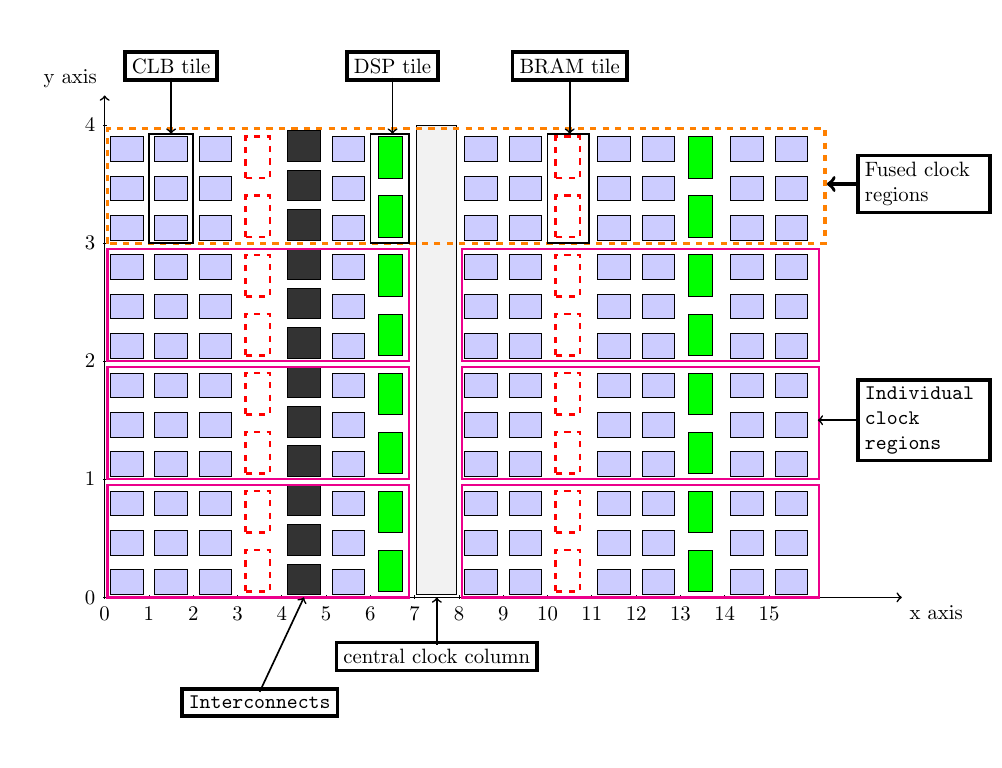
\includegraphics[width=\linewidth]{graphics/fpga.png}
  \caption{FPGA architecture}
  \label{fig:fpga}
\end{figure}

Partially reconfigurable applications are often composed of \textbf{\textit{M$_s$}} number of static and \textbf{\textit{M$_r$}} number of reconfigurable modules that are to be placed in \textbf{N$_s$} static and \textbf{N$_r$} reconfigurable regions on the FPGA respectively.  In PR applications the number of static modules equals to the number of static regions i.e., \textit{M$_s$ = N$_s$} while the number of reconfigurable modules is always greater than reconfigurable regions i.e., \textit{M$_r$ $>$ N$_r$}. Floorplanning in PR can then be defined as the process of allocating placement for \textit{N$_r$} reconfigurable regions on the FPGA fabric. \\

\textbf{state how PR-fp is currently done in vivado} \\

\subsection{Combining clock regions}
On Xilinx FPGAs, the central clock column divides the FPGA into left and right regions as shown on fig \ref{fig:fpga}. But in our model all the horizontally adjacent clock regions were fused into a single clock region. This simplifies our modeling with no penalty. As also shown in the figure on fig \ref{fig:fpga}, a cartesian coordinate system can be overlayed on FPGAs to uniquely identify each resource on the logic fabric. The x axis represents each column of resources while the rows on the y axis represent the fused horizontally adjacent clock regions as indicated on fig \ref{fig:fpga}. Combining the horizontally adjacent clock regions\footnote{henceforth clock regions implies horizontally fused clock regions}, in addition to resulting in a lower range of variables on the y axis, organizes resources on the y axis on a per tile (per clock region) basis instead of as individual clbs, brams or dsps. This reduces the search space for the solution in the MILP formulation at the expense of wasting resources. Based on this abstraction the resources on the FPGA fabric on a tile basis, the FPGA would become \textbf{W} columns wide and \textbf{H} clock regions high.  \\

The i\textsuperscript{th} reconfigurable region R$_i$ is a rectangular region on the FPGA fabric that hosts, at different durations, the set of reconfigurable modules assigned to it. R$_i$ can be represented as
\begin{equation}
R_i = (x_i, y_i, w_i, h_i) \mid x_i + w_i \leq W, y_i + h_i \leq H
\end{equation}

where x$_i$ and y$_i$ represent the bottom left coordinate and w$_i$ and h$_i$ represent the width and height of R$_i$ resectively. A resource type \textit{t} that is required by reconfigurable module \textit{M$_r$} is denoted as \textit{c$_{rt}$} while the same type of resource that is incorporated inside a reconfigurable region R$_i$ is denoted as $\eta_{it}$. The upper and lower boundaries of R$_i$ are aligned to clock region boundaries since the resources on the fabric are organized on a tile basis. 

\textbf{\\talk about the modeling of forbidden regions}

\subsection{Discretization of the axis}
Floorplanning is a two dimensional (quadratic) problem in that determining the number of resource contained in R$_i$ invloves determining the resources on both axis i.e., the area of the rectangle. To linearize this problem either of the axis must be discretized. A good strategy for discretization would be choosing the axis with the lower range of variables as this leads to an easily scalable model. In all the FPGA families that were chosen to be studied for this project, the range of the y axis (the number of clock regions on the y axis) was less than the range of the x axis i.e., H $<$ W. For example in kintex xc7z045fbv676 there are 100 columns on the x axis as opposed to 7 clock regions on the y axis. Hence the binary variable $\beta_{ij}$ denotes clock region j in region in R$_i$. \\

%$\forall$ i = 1...,N$_r$,  $\forall$ j = 1...,H \\
%$\beta_{ij}$ $\in$ [0,1] $\mid$ $\beta_{ij}$ represents clock region j in R$_i$. \\

\subsection{FPGA resource finger-printing} 
Resources in most Xilinx FPGAs are distributed in a redundant manner this is to say vertically adjacent clock regions have a fairly similar distribution of resources with the possibility of different forbidden regions being included in them. Hence the reconfigurable fabric of most Xilinx FPGAs can accurately be represented by describing the resources in a single clock region and the location of forbidden regions in all clock regions. This process is equivalent to developing the resource distribution finger-print of a specifc type of FPGA. For each resource type \textit{t} a piecewise function f$_t$(x) can be used to describe the distribution of that particular resource inside the first clock region of the FPGA along the x axis. As an example f$_t$(x) for the first clock region on fig \ref{fig:fpga} would be 

\begin{figure}
  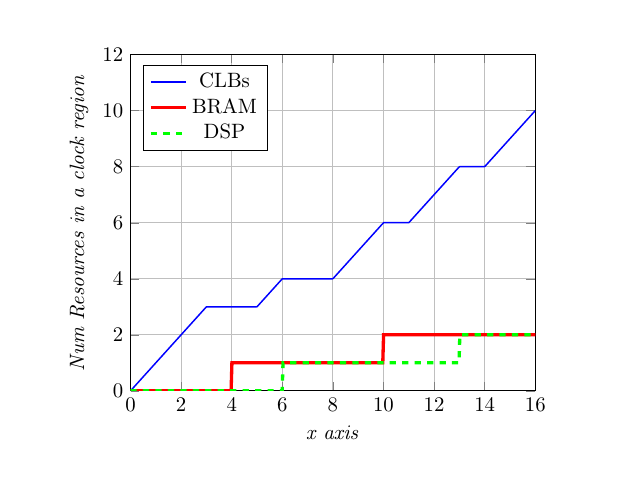
\includegraphics[width=\linewidth]{graphics/resource.png}
  \caption{Resource distribution finger print of fig \ref{fig:fpga}}
  \label{fig:finger-print}
\end{figure}


\begin{comment}
\begin{equation}
f_c(x) = \begin{cases}
\mu_c * x, & \textbf{ 0$\leq$x$<$4}, \\
\mu_c * (x-1), & \textbf{4$\leq$x$<$7}, \\
\mu_c * (x-2), & \textbf{7$\leq$x$<$W}, \\
\end{cases}
\end{equation}
\end{comment}

%\textbf{fig} depicts f$_t$(x) for the first clock region zynq xc7z015.

If $\mu_t$ is a constant that denotes the number of resource \textit{t} per tile, the amount of each type of resource included inside a region R$_i$ i.e., $\eta_it$ can be defined as \\

\begin{equation}
\label{model:eq:4}
\eta_{it} = \sum_{j=1}^{H} \beta_{ij} \cdot (f_t(x_i+w_i) - f_t(x_i)) * \mu_t
\end{equation}

\begin{comment}
The set of components that must not be included in 
A reconfigurable region R$_i$ must, at the very least, incorporate the resources required by the largest reconfigurable module that it hosts. Reconfigurable regions are rectangular in shape and to ease the routing during implementation, the height of the reconfigurable region must be aligned to clock region boundaries.\\
\end{comment}
